% !TeX root = ../main.tex

\chapter{学习画像}
\label{sec:profile-path}

\section{学习画像总体架构}

口腔医学学习具有知识依赖密集、概念边界细致、诊疗决策链条长的特点。同一疾病的知识点下往往同时涉及解剖基础、病因机制、临床表现、诊断依据、治疗原则和预后维护。OralSage 因此将学习画像设计为贯穿学习过程的共享状态模型，用于连接课程规划、讲授组织、上下文问答、阶段测评和学习计划推荐。画像记录学习者当前希望达成的目标，也记录系统在交互中逐步观察到的知识状态、解释偏好和执行节奏，使每一次后续决策都能建立在可复用的个体信息之上。

参考智能教学系统中学习者建模与知识追踪的基本思想\cite{corbett1994knowledge,vanlehn2011relative}，与近期智能体个性化辅导研究中“静态知识基础+动态个人记忆”的分层理念\cite{deeptutor2026}，OralSage 以口腔医学知识图谱组织课程知识与学习单元，以学习事件和多层记忆记录学习者的学习行为，并在持续交互中动态更新学习画像。面向具体学习任务时，系统再通过角色化画像切片，将与当前主题和 Agent 职责相关的信息按需交付，为课程规划、讲解、答疑、测评和计划推荐提供个性化依据。

\begin{figure}[H]
  \centering
  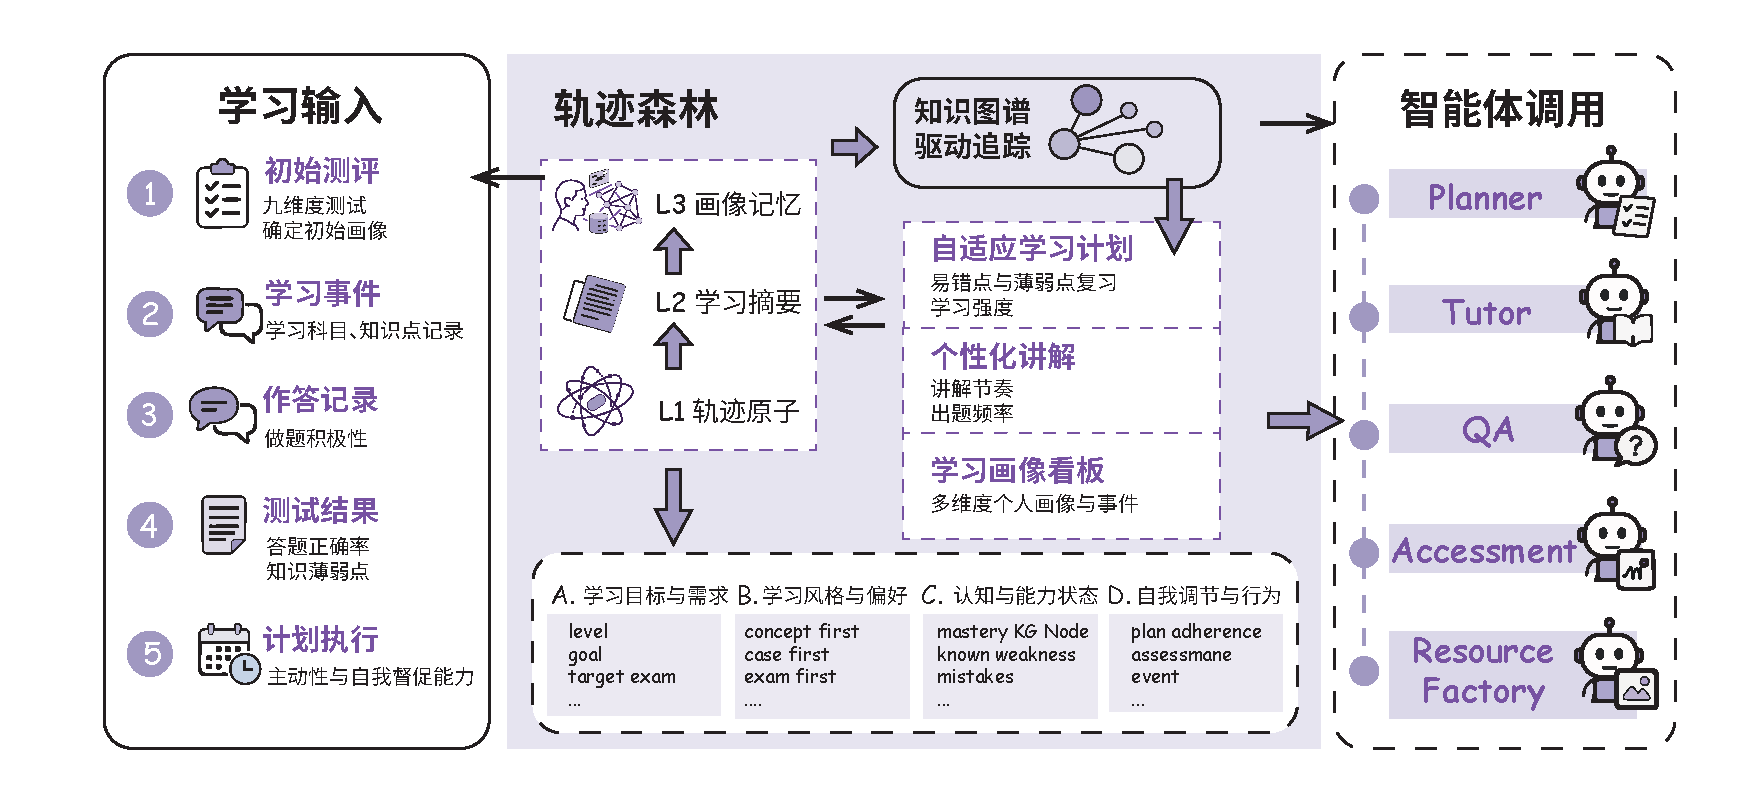
\includegraphics[width=\linewidth]{figures/profile-overall-architecture.pdf}
  \caption{OralSage 学习画像总体架构}
  \label{fig:profile-overall-architecture}
\end{figure}

如图\ref{fig:profile-overall-architecture}所示，OralSage 将初始测评、课程讲授、追问、答题、阅读、复习和计划打卡等学习事件存入持久化学习记忆中，经由按学习轨迹聚合的摘要形成较为稳定的行为描述，最终通过 LLM 总结写入长期记忆，形成动态更新的学习画像，并且支持产品侧的响应速度与长期行为建模保持协同。

\section{初始画像构建与教学调节}

\subsection{初始测评}

学习者首次进入学习流程时，OralSage 将提供九道测评题目，围绕学习目标、每日可用时间、知识进入方式、讲解深度、学习节奏、小测接受度、计划引导需求、时间紧张时的优先策略和自动调整接受度几个维度来采集用户的偏好信息，为个性化服务提供基础。测评结果写入基础画像，并生成解释深度、知识进入方式、互动倾向、节奏和计划支持需求等风格维度。系统据此生成考试导向、练习驱动、病例驱动、机制推导等学习者类型描述。

\begin{table}[H]
  \centering
  \caption{初始测评维度与学习调节映射}
  \label{tab:onboarding-profile-mapping}
  \begin{tabularx}{\linewidth}{p{0.22\linewidth}p{0.30\linewidth}X}
    \toprule
    测评维度 & 主要画像字段 & 后续调节作用 \\
    \midrule
    学习目标 & 学习目标、目标考试 & 路径重点与任务优先级 \\
    每日时间 & 每日可用时间、节奏 & 每日任务量与计划周期 \\
    知识进入方式 & 讲解偏好、进入方式 & 概念、病例、题目和考点的组织顺序 \\
    讲解深度 & 解释深度 & 机制讲解与要点归纳的展开程度 \\
    小测接受度 & 测评偏好 & 小测密度与阶段练习安排 \\
    计划引导需求 & 计划支持需求 & 任务拆分粒度与推荐强度 \\
    时间紧张策略 & 复习需求、目标倾向 & 重点复习与主线推进的权重 \\
    自动调整接受度 & 执行节奏、计划偏好 & 计划变更的呈现方式与调整频率 \\
    \bottomrule
  \end{tabularx}
\end{table}

\subsection{面向口腔医学任务的支架化调节}

支架化教学与维果茨基提出的“最近发展区”思想密切相关，强调辅导系统应依据学习者的当前状态提供适度支持，并随着学习进展调整支持强度\cite{wood1976tutoring}。OralSage 将这一思想落实为共享学习状态驱动的协同调节机制。系统在课程范围、知识点优先级、讲解组织、答疑补充、测评反馈和任务密度等决策中读取同一份学习画像，根据学习目标确定课程重点，根据知识掌握状态调整讲解与复习内容，并结合可用时间和执行节奏调节任务密度，使不同学习环节围绕学习者当前状态保持协调，并在后续交互中持续调整支持方式。

OralSage 的这种动态调节将学习偏好视为可被持续校准的工作假设。用户后续的追问方式、答题反馈和计划执行能够逐渐补充对学习行为的理解，并逐步形成更加稳定的学习画像。因此，系统能够在较短学习任务中保持一致的讲解策略，也能够在跨会话学习中根据长期表现调整节奏和任务密度。

\section{轨迹森林与多层学习记忆}

\subsection{从学习事件到长期画像}

为处理跨课程、跨会话的连续学习记录，OralSage 构建了“轨迹森林”式的多层学习记忆。系统将学习者在不同课程和会话中产生的学习事件分别组织为持续延伸的学习轨迹，多条轨迹共同构成反映长期学习过程的“轨迹森林”。该结构围绕问答、讲授、测评、规划、阅读、复习和学习计划等学习行为，将细粒度的事件逐步归纳为可调用的长期状态。L1、L2 与 L3 的层级关系如图\ref{fig:trace-forest-flow}所示。

\textbf{L1 学习轨迹原子层}以 \texttt{lesson\_events} 保存课程学习、授课推进、用户追问、答题提交、进度更新、资源阅读、复习完成和计划执行等学习事件，并关联 KG 节点、行为结果和上下文信息。

\textbf{L2 学习摘要层}以 \texttt{learning\_summaries} 对同类事件进行阶段性归纳。摘要能够捕捉画像关键变化、关联 KG 节点和来源事件编号，避免下游模块反复读取大量原始交互记录。\texttt{memory\_consolidation\_meta} 保存已处理事件的位置，使归纳过程可按新增事件持续推进。

\textbf{L3 长期画像记忆层}将阶段性摘要和有效学习行为整理为六个维度的画像字段，分别覆盖总体特征、知识掌握、薄弱点、学习偏好、目标和节奏。\texttt{profile\_state} 进一步汇总学习风格、薄弱点与易错点、知识点掌握度和个性化策略。

\begin{figure}[H]
  \centering
  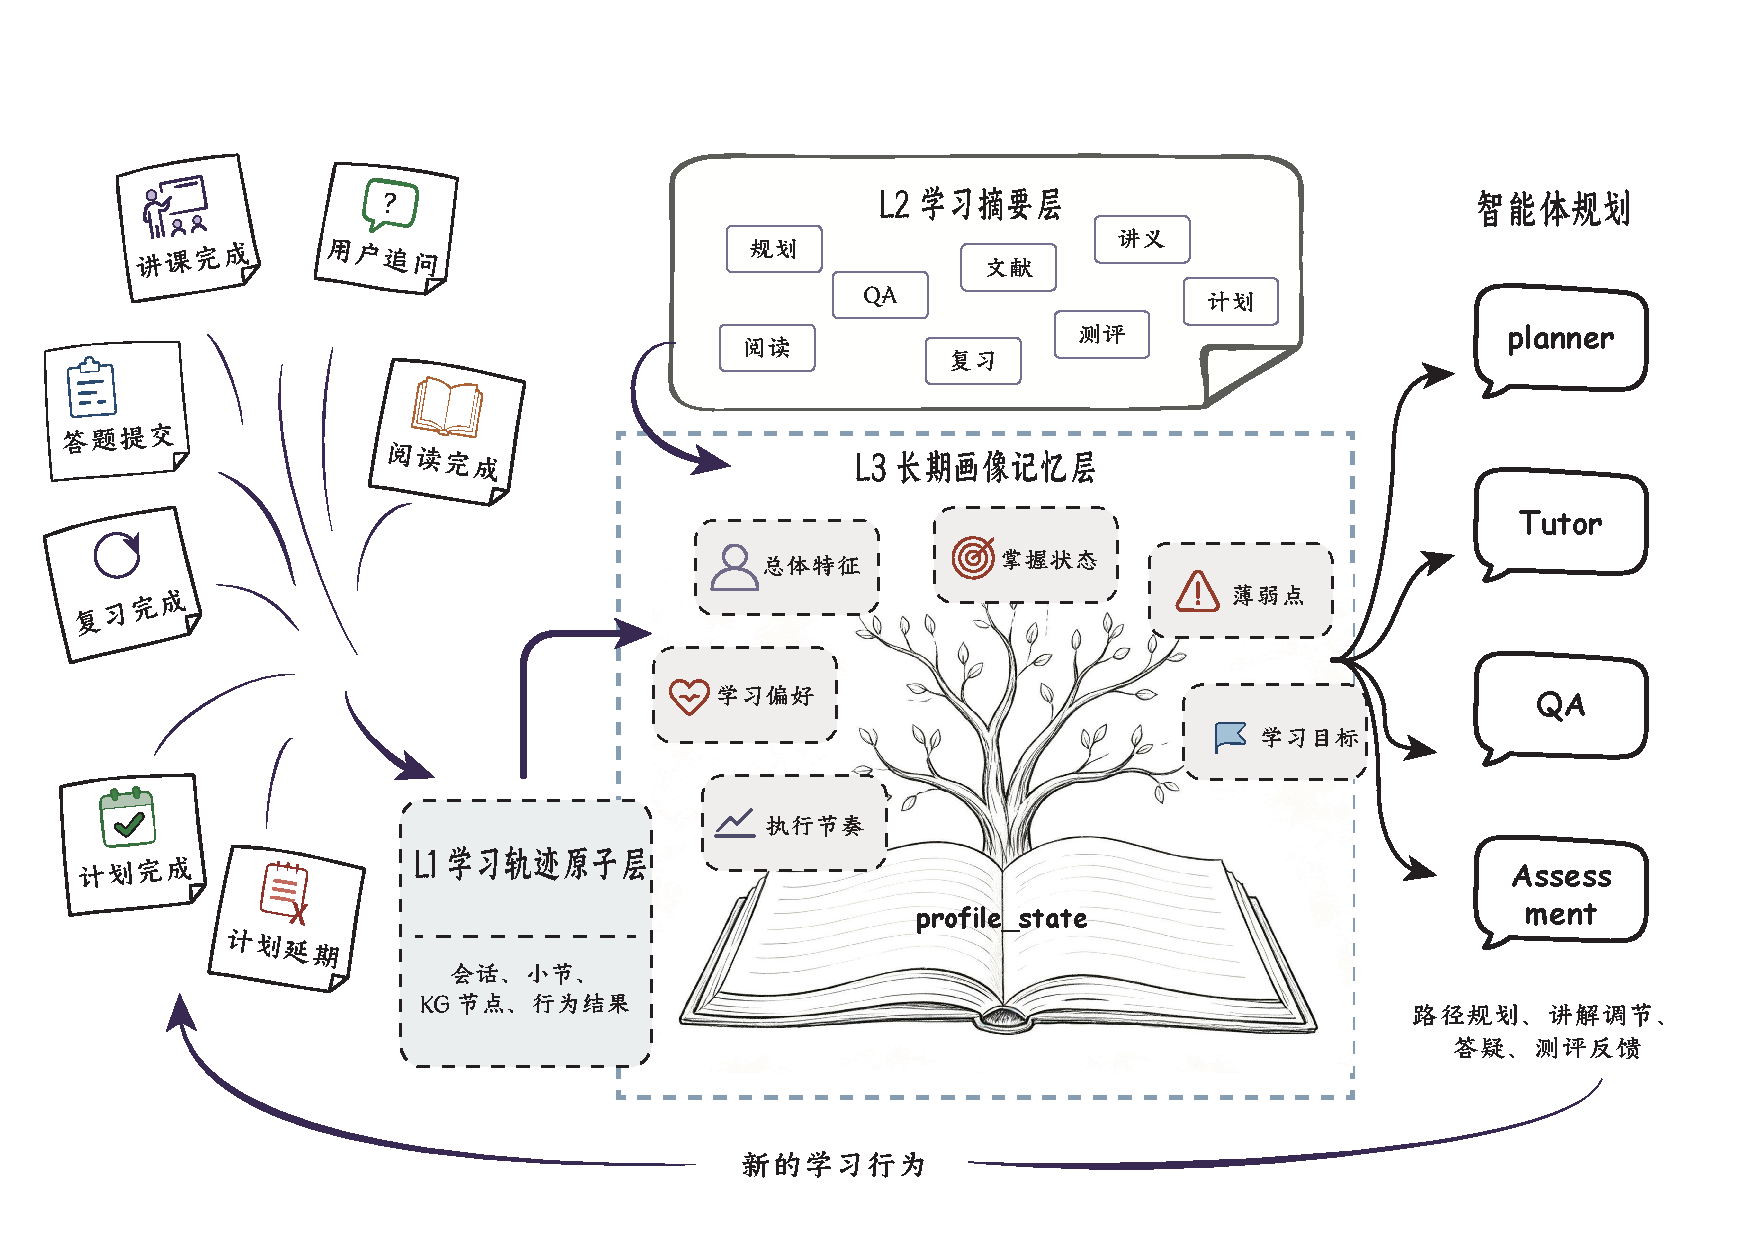
\includegraphics[width=0.96\linewidth]{figures/trace-forest.pdf}
  \caption{轨迹森林三层协作流程}
  \label{fig:trace-forest-flow}
\end{figure}

\subsection{学习画像的动态更新}

OralSage 能够将“用户说过什么”“用户做过什么”“据此形成何种判断”和“用户是谁”连接为完整的记录链。学习事件存入 L1 后，系统对事件进行语义归类，记录相应的记忆类别、画像维度、行为内容和关联 KG 节点；随后通过事件编号与有效性校验，将同类事件逐步归纳为阶段性摘要。只有经过持续学习行为支持、能够形成相对稳定判断的信息，才会进一步进入长期画像。长期画像中的特征并非一次写入后永久固定，而是能够随着后续行为被新增、修订、强化或减弱。对于掌握度与薄弱点，系统会保存用户答题分值，并结合后续学习表现更新相关知识点的掌握状态与错误理解程度。

\subsection{数字问诊事件与画像反馈}

数字问诊使用独立事件类型记录临床训练轨迹。\texttt{clinical\_speaking\_started} 保存病例训练启动信息，\texttt{clinical\_diagnosis\_confirmed} 保存诊断确认结果，\texttt{clinical\_speaking\_answer\_assessed} 记录病理机制、临床表现与诊断依据、鉴别诊断、治疗原则、风险与随访的分项得分，\texttt{clinical\_speaking\_completed} 汇总总分与完成状态。这些事件在画像时间线中以“问诊、诊断、考核”呈现，学习者可以通过问诊筛选查看相关活动。

判官 Agent 的分项结果会更新相关知识节点的掌握度、接触次数和置信度，回答中遗漏的关键内容同步进入已知薄弱点。画像保留目标诊断、领域名称、得分、遗漏要点和会话来源，使一次表达不足能够定位到具体知识内容。新建问诊会话时，病例选择服务读取 \texttt{known\_weak\_points} 与近期学习主题，将已有学习记录转化为优先训练方向，完成“训练表现、画像变化、再次选题”的连续循环。

由于学习目标、可用时间、讲解偏好和任务执行策略会随课程阶段发生变化，OralSage 将这一现象建模为\textbf{学习偏好漂移}（learner preference drift），并据此构建时变学习者画像。时间感知推荐研究表明，用户兴趣与行为模式具有明显的时间动态，较早观察对当前偏好的解释力会逐步减弱\cite{koren2009temporal}。在口腔医学学习场景中，系统学习、考前冲刺和查缺补漏等阶段对内容组织与任务密度的需求并不相同，因此画像聚合需要持续关注近期学习行为，该设计能够降低一次短暂偏好对长期画像的影响，同时保留反复出现的稳定行为特征。

设某条记忆距当前时间为 $\Delta t$ 天，其时间权重定义为：
\begin{equation}
  w_t=\max\left(0.25,\ 0.5^{\Delta t/90}\right).
  \label{eq:profile-recency}
\end{equation}

其中，画像信号的减半周期设置为90天，使置信度与时间权重共同影响风格和状态的汇总，并通过 0.25 的下界保留长期目标、持续性薄弱点和稳定偏好的基础影响，适合处理学习者在备考冲刺、课程切换等场景中的短期行为波动。

\section{角色画像切片与 Agent 调用}

完整学习画像包含较多历史信息，若所有模块都读取全部内容，会显著增加上下文负担，也会导致当前任务最关心的部分被淹没。因此，OralSage 构建 Profile Slice 机制。系统根据Agent角色、当前主题、小节和关联 KG 节点提取小型画像子集，并优先保留与当前知识节点相关的掌握度和薄弱点记录。存在会话上下文时，切片还会附带近期学习摘要，使智能体能够理解当前学习阶段。具体按需调用的画像切片内容与决策影响如表\ref{tab:profile-slices-agents}所示。

\begin{table}[H]
  \centering
  \caption{智能体的画像切片与决策影响}
  \label{tab:profile-slices-agents}
  \begin{tabularx}{\linewidth}{p{0.18\linewidth}p{0.42\linewidth}X}
    \toprule
    调用模块 & 主要切片内容 & 决策影响 \\
    \midrule
    Planner & 目标、每日时间、节奏、薄弱点、KG 节点掌握度、近期学习摘要 & 路径范围、小节顺序、任务密度与复习插入位置 \\
    Tutor & 解释偏好、知识进入方式、节奏、当前节点掌握度与薄弱点 & 讲解入口、例证组织、展开深度和小测提示 \\
    QA & 近期困惑、表达偏好、相关 KG 节点、掌握度与薄弱点 & 答疑角度、补充解释范围和是否需要加强复习 \\
    Assessment & 答题历史、错因摘要、薄弱点、掌握度与节奏 & 评分反馈、错因解析和补救建议 \\
    综合考试工具 Agent & 薄弱知识点、掌握记录、近期作答表现与目标考试 & 单选题优先级、简答题知识侧重与复习内容更新 \\
    Study-Planner & 掌握状态、待完成任务、延期记录、错题记录和执行节奏 & 继续学习、复习、练习、自测和补计划任务 \\
    \bottomrule
  \end{tabularx}
\end{table}

综合考试调用画像切片时，仅保留与命题有关的知识状态和学习目标。服务依据这些信息优先选择与薄弱内容相关的题库题目，并将同一份切片作为讯飞星火生成简答题时的知识侧重信息。考试结果中的单选得分、简答题反馈和缺失要点随后进入学习记录，后续复习推荐能够读取这一轮考试留下的细粒度表现。

\section{知识图谱约束的知识状态追踪}

知识追踪的关键在于将学习行为映射到明确的知识单元，并持续更新该单元的掌握状态\cite{corbett1994knowledge,piech2015deep}。OralSage 以口腔医学知识图谱节点作为课程学习单元，将课程大纲、讲义小节、题库和学习事件通过 KG 节点关联到同一知识空间，使“系统已讲授的内容”“用户作答的题目”“用户反复追问的概念”能够在同一节点尺度上汇合。

当前实现采用面向业务可解释性的掌握记录机制。系统围绕用户、会话和 KG 节点汇聚讲授覆盖、测评作答与问答困惑等学习信息，并在 \texttt{mastery\_records} 及直接问答掌握记录中保存掌握分数、置信度、讲授次数和关联上下文。各类行为依据其诊断价值写入不同幅度的状态增量，明确困惑同步进入薄弱点记录。该机制将分散的学习过程收束为节点级知识状态，为后续复习推荐、定向练习和个性化答疑提供统一输入。

\begin{figure}[H]
  \centering
  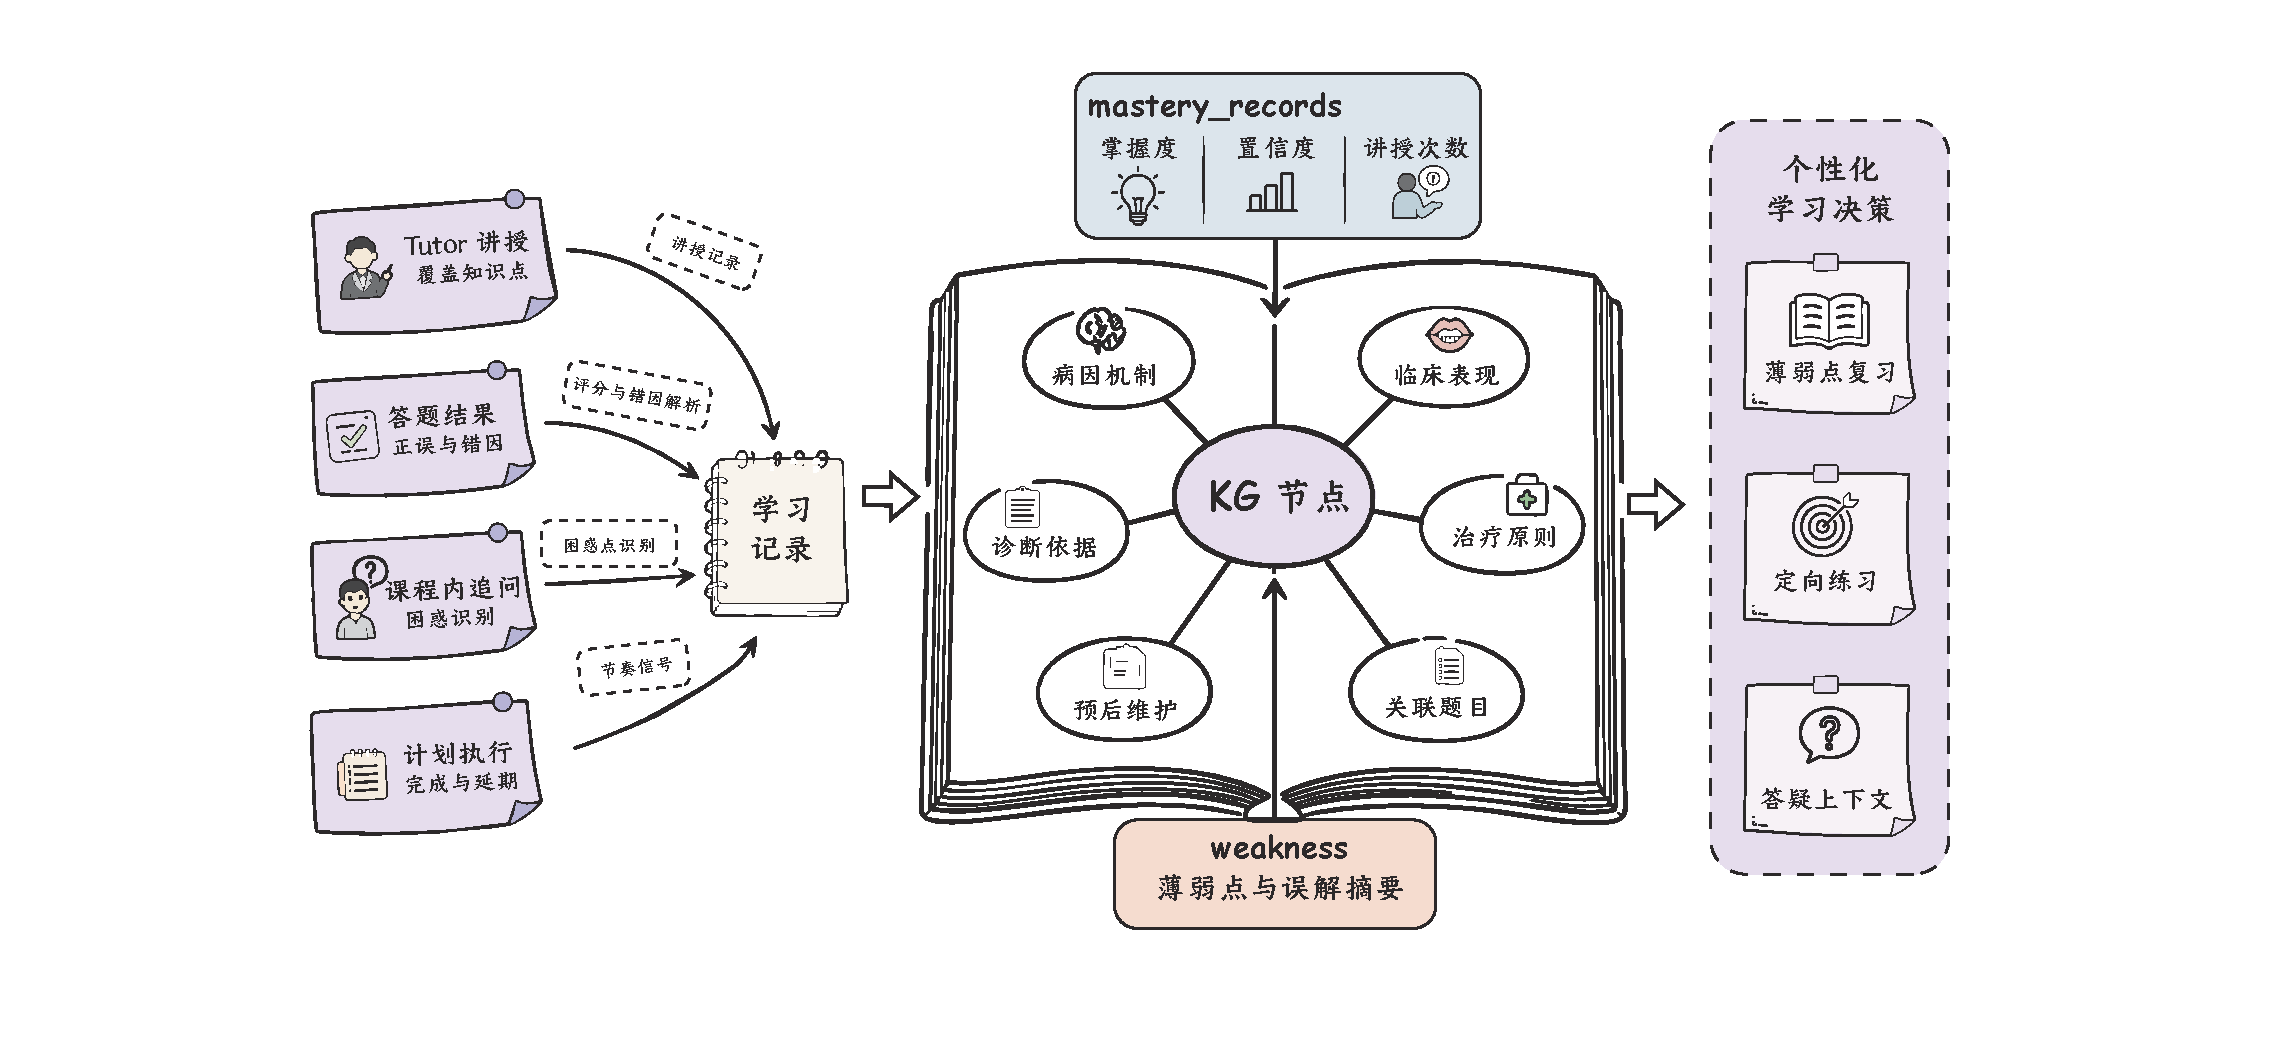
\includegraphics[width=0.94\linewidth]{figures/KG-knowledge-trace.pdf}
  \caption{学习行为与 KG 节点关联流程}
  \label{fig:learning-behavior-to-kg}
\end{figure}

如图\ref{fig:learning-behavior-to-kg}所示，知识图谱能够发挥课程组织和学习状态定位的双重作用，在为路径规划提供概念依赖与章节边界的同时，让薄弱点回顾、定向练习和答疑上下文能够聚焦到相关知识单元。相较于只记录总正确率的方式，节点级追踪能够进一步识别学习者对哪些具体知识内容掌握不足，更适合口腔医学中诊断条件、疾病分期、适应证与治疗原则容易发生混淆的学习任务。具体行为对后续学习状态的影响如表\ref{tab:learning-behavior-effects}所示。

\begin{table}[H]
  \centering
  \caption{主要学习行为对画像与知识状态的影响}
  \label{tab:learning-behavior-effects}
  \begin{tabularx}{\linewidth}{p{0.20\linewidth}p{0.34\linewidth}X}
    \toprule
    学习行为 & 主要记录内容 & 画像与状态更新 \\
    \midrule
    Tutor 讲授 & 小节、覆盖 KG 节点、讲授次数 & 写入 \texttt{tutor\_exposure}，形成小幅掌握度与置信度增量 \\
    答题正确 & 题目、关联节点、评分结果 & 提升对应节点的掌握度，并更新课程进度 \\
    答题错误 & 错选原因、误解摘要、关联节点、补救建议 & 降低相关节点掌握度，写入薄弱点和错因模式 \\
    课程内追问 & 问题、上下文、困惑节点、答疑结果 & 对明确困惑写入薄弱点与问答掌握记录，扩展性提问保留为交互记录 \\
    数字问诊 & 诊断结果、五域分数、遗漏要点、关联知识节点 & 更新掌握度、接触次数、置信度与薄弱点，并影响后续病例选择 \\
    计划完成或延期 & 任务状态、日期变化、完成情况 & 写入节奏类记忆，为后续任务密度和优先级调整提供输入 \\
    \bottomrule
  \end{tabularx}
\end{table}

\section{掌握学习反馈循环}

根据掌握学习理论指出的测评后的针对性反馈与补救机会能够帮助学习者逐步达成预设学习目标\cite{bloom1968mastery}的思想，OralSage 设计“测评、分析、反馈、再练习、再规划”的连续循环。Assessment 能够对学习者提交的错误答案，结合讲义小节和关联知识节点提供正确答案解释，生成错选原因，总结误解摘要，为学习者提供复习和知识补救建议。随后，相关知识节点的掌握状态和薄弱点记录进入学习画像，并供后续讲解、问答和计划推荐使用。

\begin{figure}[H]
  \centering
  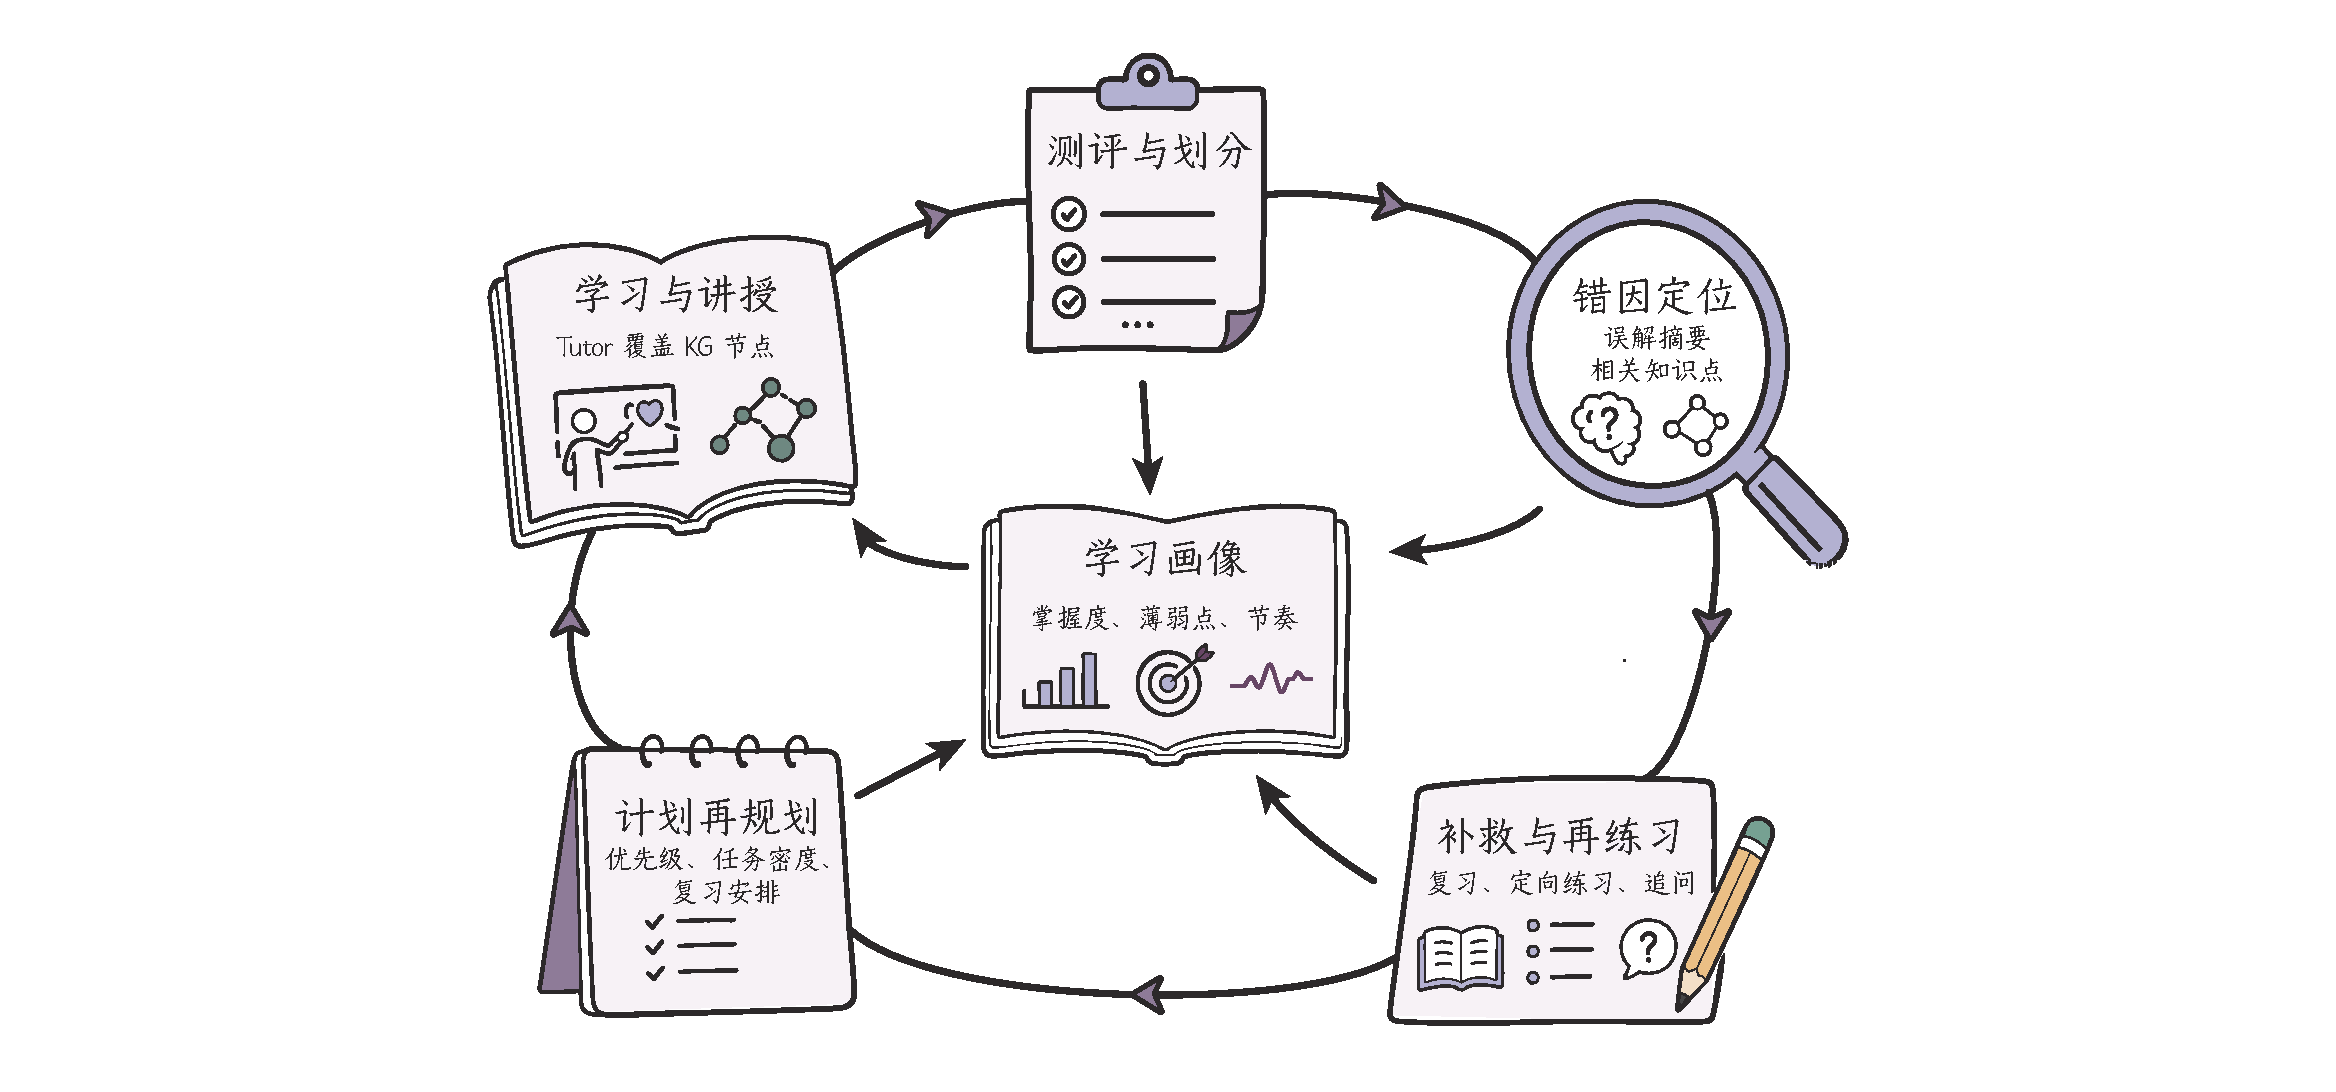
\includegraphics[width=0.94\linewidth]{figures/profile-feedback-loop.pdf}
  \caption{掌握学习反馈循环}
  \label{fig:mastery-feedback-loop}
\end{figure}

如图\ref{fig:mastery-feedback-loop}所示，反馈循环的重点在于将补救行动重新写入学习轨迹。学习者完成薄弱点复习、定向练习或阶段测评后，新的行为事件会进入 L1 层，经过摘要和长期记忆更新影响下一次学习决策。系统由此能够将一次答错转化为后续课程中的可执行任务，并持续组织相应的复习安排。

\section{画像可视化}

学习画像页将抽象的学习状态转化为学习者易于理解的可视化界面。页面展示近期学习天数、本日计划、完成记录、每日可用时间和学习活动趋势，并通过能力雷达图呈现自主规划、执行反馈、学习节奏、薄弱点修正、知识掌握和练习反馈等维度；当前学习风格、易错点与错因、目标导向、学习偏好及事件时间线也会在同一页面集中呈现。这些信息不仅用于展示学习结果，也帮助学习者理解近期完成了哪些任务、哪些知识仍需巩固，以及当前学习安排依据何种状态形成。

此外，用户可以重新完成测评来更新偏好基线，系统能够实时记录历史学习行为和知识状态。通过学习趋势、易错点和事件时间线，学习者可以回顾自身状态的变化；通过重新测评和学习计划入口，学习者也可以对原有偏好与后续安排进行调整。画像可视化由此不仅承担结果展示功能，也在系统的个性化判断与学习者的自主决策之间建立可理解、可回顾和可调整的交互界面。
